\documentclass[a4paper]{article}
\usepackage[utf8]{inputenc}
%\usepackage[a4paper, total={150cm, 250cm}]{geometry}

\usepackage{tikz, sidecap, graphicx}
\usetikzlibrary{positioning, shapes}

\usepackage{geometry}
 \geometry{
 a4paper,
 total={150mm,257mm},
 left=30mm,
 top=20mm,
 }



\title{Report week 6}
\author{Bård-Kristian Krohg \\ \texttt{baard.krohg@gmail.com}}


\begin{document}
\maketitle

\section{Speeding up rendering}
\begin{itemize}
\item Tested NiTE2's tracker for kinect2 (video).
\item Implemented manual method for constraining keypoints.
\end{itemize}

\subsection{Results}
To constrain the human body, we implemented a scaling function based on the weighted sum of all the observed keypoints. However, the results are varying:
\begin{table}[h]
  \centering
  \begin{tabular}{|r l|}
    \hline
    True Height: & 1.72 \\
    \hline \hline
    Average: & 1.84 \\
    Median: & 1.49 \\
    Average deviation from median: & 0.51\\
    \hline
  \end{tabular}
  \caption{Results from approximatley 2 seconds of observation where the subject is standing still with a clear view to all keypoints.}
\end{table}

Some other problems were also discovered, such as if a keypoint between two well observed keypoints is not observed well, we should have a method to calculate where this keypoint \emph{should} be given the scaled lengths of the limbs between the keypoints.

\begin{figure}[h]
  \centering
  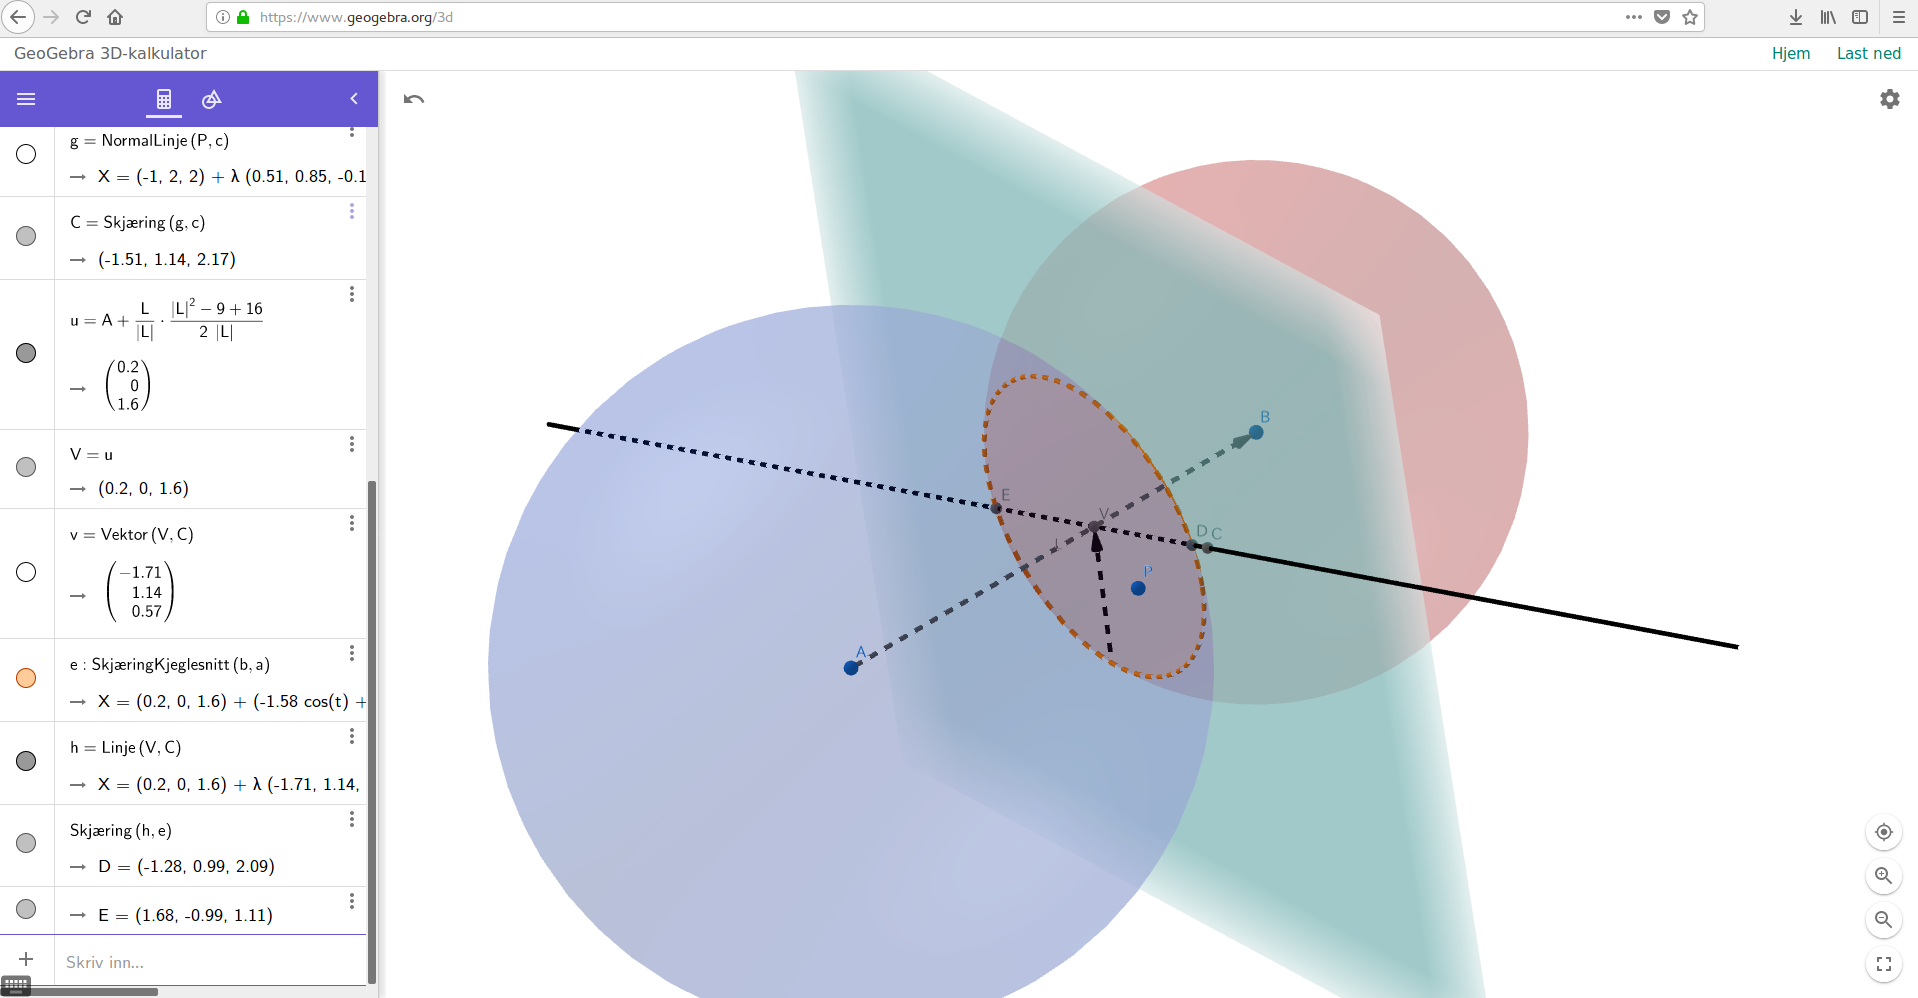
\includegraphics[width=.95\textwidth]{lensnearestpoint}
  \caption{The candidates (D,E) for the estimated position of a not-well-observed point P between two well observed points A,B. C is the point P projected into the plane created between the intersection of the spheres around A,B with radius equal to the respective wanted limb lengths.}
\end{figure}

\subsection{Observations}
\begin{itemize}
\item The NiTE2 program seems to use a skeleton with \emph{fixed} lengths, although it is scaled to the person.
\item It looks like the software produces a full 3D skeleton as long as enough keypoints are tracked.
\item Direct data from the NiTE2 seems to be a little unstable. For games, this data is probably filtered.
\item NiTE2 seems to track best between 160 -- 400 cm from the sensor.
\end{itemize}

\subsection{Problems/Next week}
\begin{itemize}
\item The code for manually refining the 3D keypoints is still a little buggy/unfinished. I would like to look into creating a ML model for estimating the 3D keypoints, since this is what the NiTE2 software uses.
\item Complete tracking of each person based on CoM of the observed keypoints.
\end{itemize}
\begin{figure}[b]
  \centering
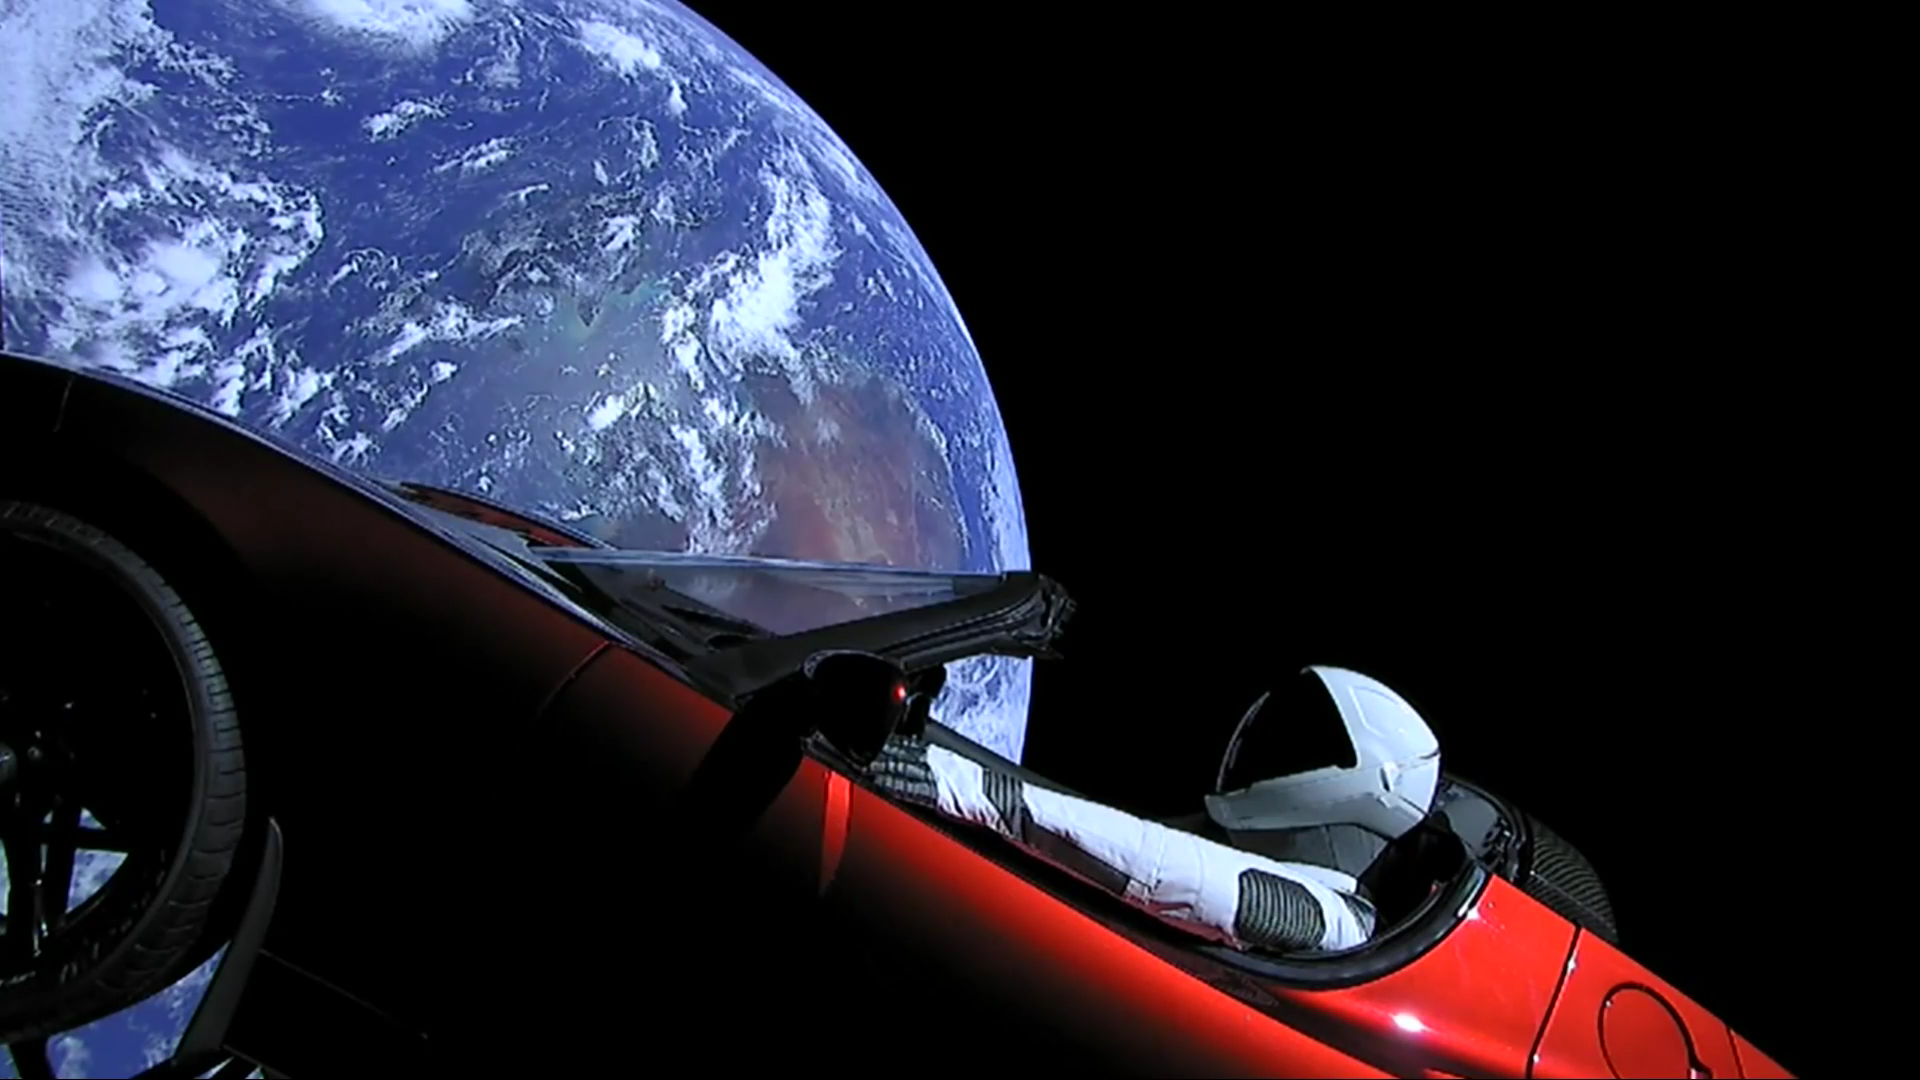
\includegraphics[width=.75\textwidth]{starman}
\end{figure}
\end{document}

